\section{Formal Semantics}
\label{sec:formalisation}

%% First update reasoning cycle states...

Briefly, these are the changes in the semantics of AgentSpeak(L)
that are needed to accomodate the new features of AgentSpeaker(ER):

\begin{itemize}
\item in the beginning of the reasoning cycle, check all
  goal-conditions starting from the bottom of each intention stack and
  remove all finished intentions;

\item if an event is \emph{external}, try to trigger one
  applicable plan for each intention, starting from the
  top of the intention stack (that is, the most specific plan in the
  respective g-plan tree);

\item if an event is \emph{internal}, search for an applicable plan on
  the path to the root of the g-plan tree, that is, starting from the
  most specific plans in the g-plan tree (as in the item above but now
  there is only one intention to refer to); this does not change the
  semantics per se, only the way in which we look for relevant
  applicable plans.
\end{itemize}

We start by updating the well-known reasoning cycle~\cite{bordini:07}
to adapt it for the initial stage of checking all goal-conditions to
remove the intentions that should no longer be active. Furthermore,
note that even though this is computationally costly, it is necessary
because not doing it at every reasoning cycle may imply the agent
missing the moment where the goal-condition became true (hence an
intention needing to be deactivated); it is also worth the
computational burden in as much as it has the various practical
programming advantages we pointed out earlier in this paper.

%% RHB: I removed this text from above, but I guess it should be in
%% the initial sections
% Recall that this can be because the goal has been achieved, has become
% impossible to achieve, or the motivation why it was adopted no longer
% applies.

The required stage for checking goal-conditions is included in the
existing $\ClrInt$ stage (which previously only removed empty
intentions) except it is now moved to the beginning of the reasoning
cycle (to ensure nothing in the reasoning cycle is done under the
assumption a deactivated intention is still active), just after the
$\ProcMsg$ stage (as the information just received from other agents
might be useful in checking for goals to be deactivated). The clearing of
intentions used to be the last part of the reasoning cycle, but
because there are no other dependencies between the first and last
stages, $\ClrInt$ might as well be done at the beginning rather than
the end. The slightly changed reasoning cycle is shown in
Figure~\ref{fig:rcaser}.

\begin{figure}[htbp]
  \begin{center}
    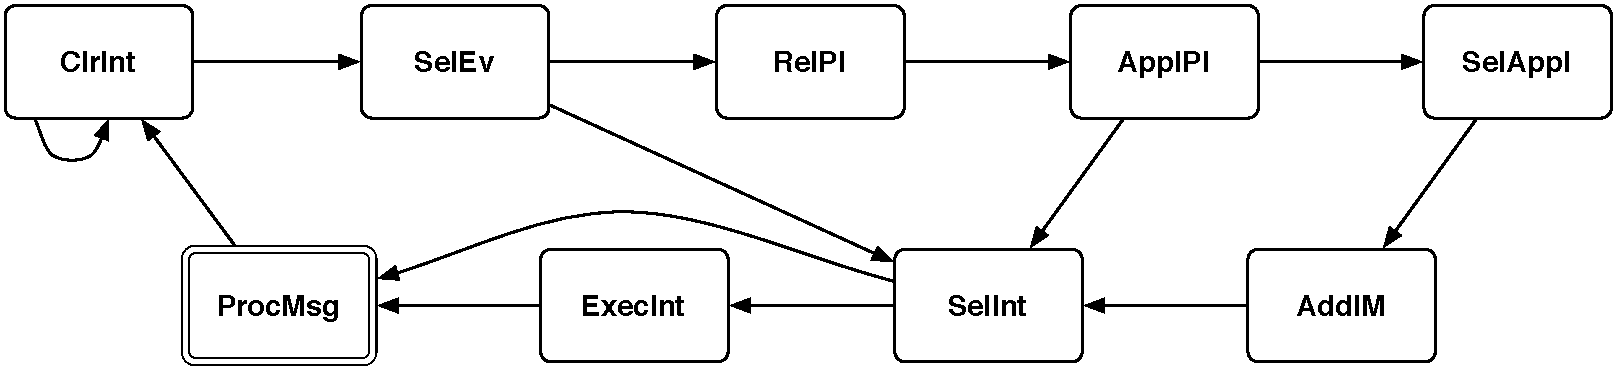
\includegraphics[width=\linewidth]{figs/ASERrc.pdf}
    \caption{The AgentSpeak(ER) Reasoning Cycle}
    \label{fig:rcaser}
  \end{center}
\end{figure}

The $\ClrInt$ stage also needs new semantic rules. In fact, the
previous 3 \rn{ClrInt} rules (see~\cite[p~212]{bordini:07}) are no
longer needed, as empty intentions are not to be removed from the set
of intentions, unless their goal condition becomes true. To facilitate
the presentation of the new rules, we define a new auxiliary function
$\GCOND$, which given a g-plan simply returns the goal-condition
component of that plan, as follows. Let $p=$``\texttt{+!g : c <: gc
  \{<- a.\}}'', then $\GCOND(p)=\texttt{gc}$, more specifically the
logical formula coded by \texttt{gc}. Also, we denote by
$[p_1,...,p_n]$ an intention stack with plan $p_n$ at its top.

The new rule \rn{ClrInt$_1$} is as shown below, and rule
\rn{ClrInt$_1$} is not shown because it simply causes the transition
$\CFG{\ClrInt} \trans \CFG{\SelEv}$ in case the negation of the
precondition of \rn{ClrInt$_1$} holds. The rule below essentially
removes from intentions the bottom-most g-plan for which its
goal-condition now follows from the state of the belief base. The
intuition is that if goal $\texttt{!g1}$ required a subgoal
$\mathtt{!g2}$ (a plan for which was pushed on top of the plan for the
former one in the intention stack) and $\texttt{!g1}$ is no longer
active, that whole part of the intention stack above it needs to be
removed together with it.

\infrule[ClrInt$_1$] {
        i \in \CI \qquad i=[p_1,\dots,p_n] \\
        \AGBELS \models \GCOND(p_j) \mbox{ for some } j, 1\leq j\leq n
}
%------------------------------------------------
{   \CFG{\ClrInt}  \trans  \CFGcp{\ClrInt} \\[1.2mm]  
\begin{array}{llcl}
  \mbox{\emph{where:}\quad}
     & \multicolumn{3}{l}{\mbox{$j$ is the least number in [1..n]
       s.t.}}\\
     & & & \AGBELS \models \GCOND(p_j)\\
     & \CIli & = & \CI \setminus \{i\} \cup \{[p_1,\ldots,p_{j-1}]\} \\
\end{array}
}

The auxiliary functions $\RELPLANS(\PLANS,\TE)$
$\APPLPLANS(\PLANS,\TE)$ (see Definitions~10.2 and~10.3
in~\cite{bordini:07}) can be changed to accommodate both the new g-plan
structure as well as the firing of e-plans (i.e., plans for reacting
to external events) for all intentions rather than creating a single
new separate intention as before. First, the redefined functions now
receive a set of intentions as an extra parameter; in the new semantic
rules they are called with the agent's plan library and the current
contents of the set of intentions ($\AGPLANS$ and$\CI$ in the
operational semantics, respectively). If $\TE$ is an external event,
the new parameter is used to check for applicable plans for each
individual intention plus the empty intention\footnote{The empty
  intention being included in the set of intentions in that parameter
  is useful for backwards compatibility with traditional AgentSpeak(L)
  but we do not discuss this here as it would hinder the explanation
  of the essential aspects of the proposed extension.}
$\EXT$. Besides having an extra parameter, the functions now return a
set of triples rather than a pair. We use $\TREV(p)$ to refer to the
triggering event of a plan $p$, and $\SCOPE([\PL_1,\ldots,\PL_n])$
returns all plans in the scope of the g-plan $p_n$. By ``in scope'',
we mean the plans that appear (immediately) within the braces
delimiting a g-plan (but not within its subgoals); for example the
plans for \texttt{+e1}, \texttt{+e2}, and \texttt{+!k} (but not for
\texttt{+e3}) are in the scope of the g-plan \texttt{+!g : c <: gc \{
  $\ldots$ \}} shown in the beginning of
Section~\ref{sec:infSS}. Furthermore, note that the $\SCOPE$ function
can determine the exact plan for $\PL_n$ in the forest of g-plan trees
now forming the plan library by using plans
$\PL_1,\ldots,\PL_{n-1}$. We can now formally define $\RELPLANS$:

\begin{definition}[Relevant Plans]\label{def:relplans}
  The auxiliary function to retrieve relevant plans given a plan
  library $PL$, a particular event $\TE$ of type \texttt{+l} or
  \texttt{-l} (i.e., an external event, one reacting to changes in
  beliefs rather than a goal adoption event), and a set of intentions
  $I$ is defined as
  $\RELPLANS(PL,\TE,I) = \{ \langle\PLANS,\theta,i\rangle \mid i \in
  I, i = [\PL_1,\ldots,\PL_n],$
  and
  $ps = \{ rp \mid rp \in \SCOPE([\PL_1,\ldots,\PL_j]) \mbox{ and }
  \{\TE\} \models \TREV(rp)\theta$,
  for some m.g.u.\ $\theta\}$, where $j$ is the greatest number in
  $[1..n]$ s.t.\ $ps \neq \emptyset$, or $ps=\emptyset$ if there is no
  such $j\}$. For internal events, the function returns a set
  containing a single element $\langle\PLANS,\theta,i\rangle$ where
  $i$ is the specific intention that generated $\TE$ and $\PLANS$ is
  the set of relevant plans using the same idea of scope as above for
  external events.
\end{definition}

We do not formally define the $\APPLPLANS$ function here due to space,
and given that it is trivially extended in a very similar way as in
Definition~\ref{def:relplans} for $\RELPLANS$.

Finally, we need to change the semantics so that not just one but
\emph{all} relevant e-plans are triggered, that is, one for
each active intention, and within a single intention starting from the
most specific plan (i.e., the one closest to the top of the intention
if there are relevant plans at other levels too). Most of the work was
already done in the redefinitions of the $\RELPLANS$ and $\APPLPLANS$
functions, but we still need to change the rule for processing
external events (which now change multiple intentions). Note however
that by the time we come to handle an external event with rule
\rn{ExtEv}, a single plan for each intention has already been
selected; that is, $\SO$ (the option selection function) is also
slightly redefined to work with the new structures returned by those
redefined auxiliary functions.

The new \rn{ExtEv} rule is below, and it essentially says that an
external event now potentially interrupts various intentions, provided
there are relevant and applicable plans anywhere in the g-plans
associated with each particular current intention of the agent. The
$\TRHO$ component of the transition system configuration has the
result of the application of the new $\RELPLANS$ and $\APPLPLANS$
functions.
% Recall that external events for the ``main'' goal --- the external
% events as in traditional AgentSpeak --- will now be associated with
% the empty intention \EXT in \TRHO (i.e., the result of the
% $\RELPLANS$ and $\APPLPLANS$ functions).
The chosen plan for each intention, after being applied its respective
variable substitution $\theta$, is pushed on top of that intention
(the notation used for this below is $i_j[\PL_j\theta_j]$).

\infrule[ExtEv] {
        \TEPS = \langle\TE,\EXT\rangle \qquad \TRHO =
        \{\langle\PL_1,\theta_1,i_1\rangle,\ldots,\langle\PL_n,\theta_n,i_n\rangle\}
}
%------------------------------------------------
{   \CFG{\ClrInt}  \trans  \CFGcp{\ClrInt} \\[1.2mm]  
\begin{array}{llcl}
  \mbox{\emph{where:}\quad}
     & \CIli & = & \CI \setminus \bigcup_{j=1}^{n} \{i_j\} \cup
                   \bigcup_{j=1}^{n} \{i_j[\PL_j\theta_j] \}\\
\end{array}
}

To conclude this section, we emphasise that, for the sake of space, we
here formalised only the main changes to the well-known AgentSpeak
semantics. The complete new transition system giving semantics to
AgentSpeak(ER) will appear in a longer paper.
